\documentclass{article}
\usepackage{tikz, comment}
\usepackage{pifont}
\usepackage{fontspec}
\usetikzlibrary{arrows, decorations.markings, decorations.pathreplacing}
\begin{comment}
:Title: Not defined yet
:Slug: No name yet

Description Here.........
\end{comment}
\begin{document}\centering

\def\rx{1.5}
\def\ry{0.5}
\def\a{8}

\begin{tikzpicture}[>=latex,xscale=.5*(\rx), yscale=.5*(\ry)]

\draw[->] (-1, 0) -- ({2*pi+1+0.3/(\rx)}, 0)node[right] {\small $\theta$} ;
\draw[->] (0, {-\a-2}) -- (0, {\a+2+0.3/(\ry)})node[above] {\small $r$} ;

\foreach \p/\q in {0/{3*pi/48}, {3*pi/48}/{13.5*pi/48}, {13.5*pi/48}/{19*pi/48}, {19*pi/48}/{29.5*pi/48}, {29.5*pi/48}/{35*pi/48}, {35*pi/48}/{45.5*pi/48}}
\draw[->, >=stealth', teal, samples=100, smooth, domain=\p:\q, variable=\t] 
		plot ({\t}, {(\a)*sin(3*\t r)});

\draw[teal, samples=300, smooth, domain={45.5*pi/48}:2*pi, variable=\t] 
		plot ({\t}, {(\a)*sin(3*\t r)});

\draw ({pi},{2pt/(\ry)}) -- ({pi},{-2pt/(\ry)}) node[anchor=north, xshift=0, scale=0.7] {$\pi$};
\draw ({2*pi},{2pt/(\ry)}) -- ({2*pi},{-2pt/(\ry)}) node[anchor=north, xshift=0, scale=0.7] {$2\pi$};

\draw ({-2pt/(\rx)}, {\a}) -- ({2pt/(\rx)}, {\a}) node[anchor=east] {\tiny $a$};
\draw ({-2pt/(\rx)}, {-\a}) -- ({2pt/(\rx)}, {-\a}) node[anchor=east] {\tiny $-a$};

\node[teal, scale=0.7] at ({pi}, {\a+1}) {$r=a \sin 3\theta$};

\node at ({-0.1}, 5) {\ding{192}};
\node at ({1/3*pi+0.1}, 5) {\ding{193}};
\node at ({1/3*pi-0.1}, -5) {\ding{194}};
\node at ({2/3*pi+0.1}, -5) {\ding{195}};
\node at ({2/3*pi-0.1}, 5) {\ding{196}};
\node at ({3/3*pi+0.1}, 5) {\ding{197}};

\node[scale=0.7] at ({-0.3/(\rx)}, {-0.3/(\ry)}) {$O$};

\end{tikzpicture}\hskip1cm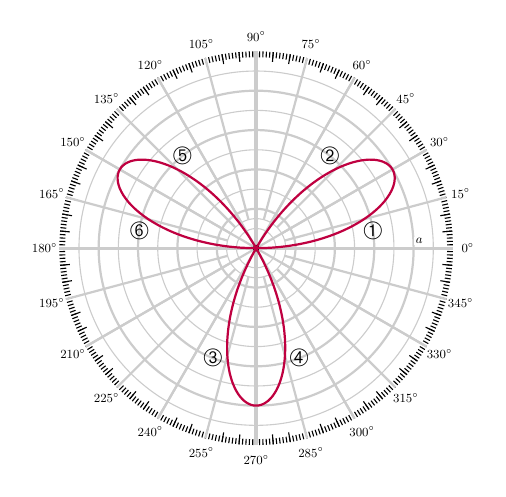
\begin{tikzpicture}[>=latex,xscale=.5*0.5, yscale=.5*0.5][font=\sf\small] 
    %Circles 
   \foreach \r in {1, 1.5, 3, 5, 7, 9}
      \draw[thin, color=gray!40] (0,0) circle (\r);
    \foreach \r in {2, 4, 6, 8}
      \draw[thick, color=gray!40] (0,0) circle (\r);   
    %1° Rays
    \foreach \a in {0, 1,...,359}
      \draw[] (\a:9.7) -- (\a:10);
    %5° Rays
    \foreach \a in {0, 5,...,359}
      \draw[] (\a:9.5) -- (\a:10);      
    %15° Rays
    \foreach \a in {0, 15,...,359}
      \draw[thick, color=gray!40] (\a:1.5) -- (\a:10); 
    %30° Rays
    \foreach \a in {0, 30,...,359}
      \draw[thick, color=gray!40] (0, 0) -- (\a:10);
    %Radius labels (background filled white)
    \foreach \r in {{5.25+2.75}}
      \draw[] ({\r},0) node[inner sep=1pt,above=1pt,rectangle,fill=white, xshift=2, scale=0.5] {$a$};
    %Main rays
    \foreach \a in {0, 90,...,359}
      \draw[very thick, color=gray!40] (0, 0) -- (\a:10);
    %Angle labels  
    \foreach \a in {0, 15,...,359}
      \draw (\a: 10.75) node[scale=0.5] {$\a^\circ$};
    %Central point
    \draw[fill=red] (0,0) circle(0.7mm/0.5);

\clip (0, 0) circle (10);

\foreach \p/\q in {0/{1*pi}}    		
\draw[purple, thick, samples=100, smooth, domain=\p:\q, variable=\t] 
		plot ({8*sin(3*(\t) r)*cos(\t r)}, {8*sin(3*(\t) r)*sin(\t r)});

\node at ({6*cos((0/3*pi+0.15) r)}, {6*sin((0/3*pi+0.15) r)}) {\ding{192}};
\node at ({6*cos((1/3*pi-0.15) r)}, {6*sin((1/3*pi-0.15) r)}) {\ding{193}};
\node at ({6*cos((4/3*pi+0.15) r)}, {6*sin((4/3*pi+0.15) r)}) {\ding{194}};
\node at ({6*cos((5/3*pi-0.15) r)}, {6*sin((5/3*pi-0.15) r)}) {\ding{195}};
\node at ({6*cos((8/3*pi+0.15) r)}, {6*sin((8/3*pi+0.15) r)}) {\ding{196}};
\node at ({6*cos((9/3*pi-0.15) r)}, {6*sin((9/3*pi-0.15) r)}) {\ding{197}};

\end{tikzpicture}
\end{document}